\documentclass[0_Bericht]{subfiles}
\setcounter{section}{3}

\begin{document}

	\section{Web Interface and Analysis Scripts}
		\subsection{Introduction}	
			Before the beginning of this semesterarbeit, an existing application was used to display all module qualification test results. As mentioned before, the main part of this semesterarbeit is to relaunch this application and adapt it to current needs, e.g. compatibility with new digital modules, more functionality, better user interface, etc.
		\subsection{Methodology}
			As a first step, a basic understanding of the CMS Pixel Detector (see section \ref{sec:LHCAndCMSPixelDetector} and the module qualification tests (see section \ref{sec:ModuleQualification}) was needed in order to analyze the requirements for the web application. In the following sections, the web interface is referred to as ``\textbf{MoRe-Web}'' (CMS Pixel Detector Module Qualification Result Web Interface).
			The general procedure was then defined to be as follows:
			\begin{itemize}
				\item Analysis of existing application
				\item Definition of Requirements
				\item Establishment of a concept for the new MoRe-Web
				\item Implemenation of MoRe-Web
				\item Testing
			\end{itemize}
			During the entire process, a repeated quality check is needed. It analyses the following aspects:
			\begin{itemize}
				\item Progress
				\item Meeting of requirements
				\item Unexpected problems
				\item Further improvements
			\end{itemize}
			
		\subsection{Analysis of Existing Application}
			The starting point of the module qualification test results is \url{http://cmspixel.phys.ethz.ch}.
			\subsubsection{BPIX Module Testing}
				At \myPath{/moduleTests/moduleDB/prodTable.php} an application called ``BPIX Module Testing'' is located. The basic purpose of this script is to display an overview table for all module qualification tests and detail pages with further information for each tested module.
				\begin{figure}[h!]
					\centering
					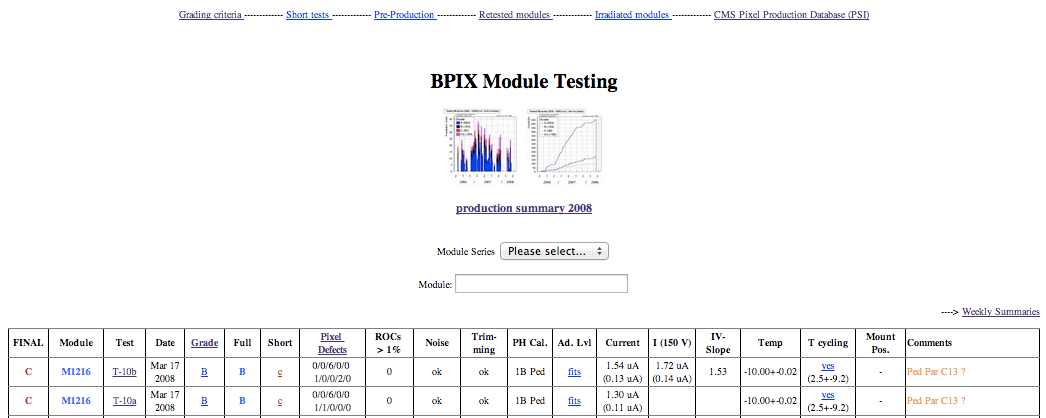
\includegraphics[width=160mm]{Content/Graphics/4_1_BPIXModuleTesting.png}
					\caption{BPIX Module Testing Overview}
					\label{fig:AnalysisOfExistingApplicationBPIXModuleTestingOverview}
				\end{figure}
				\paragraph{Frontend}
					The frontend offers an overview list of all module qualification tests as can be seen in figure \ref{fig:AnalysisOfExistingApplicationBPIXModuleTestingOverview}. 
					By clicking on a module test, an overview as seen in figure \ref{fig:AnalysisOfExistingApplicationBPIXModuleTestingROCOverview} is presented. 
					A link in the upper left corner leads to an overview graph for the module test as shown in figure \ref{fig:AnalysisOfExistingApplicationBPIXModuleTestingModuleOverview}.
					Also, there is a link horizontally centered which leads to an address levels test graph as shown in figure \ref{fig:AnalysisOfExistingApplicationBPIXModuleTestingAddressLevels}.
					By clicking a specific ROC identifier, the corresponding test results show up as given in figure \ref{fig:AnalysisOfExistingApplicationBPIXModuleTestingROCTest}.
					\begin{figure}[h!]
						\centering
						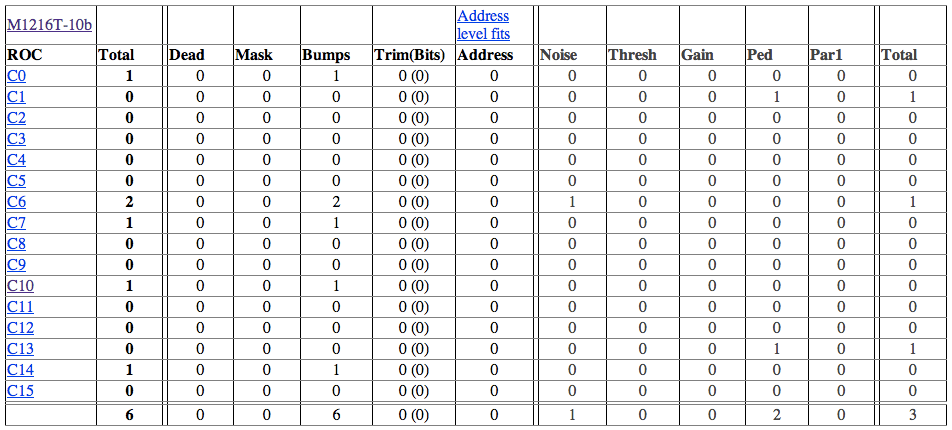
\includegraphics[width=160mm]{Content/Graphics/4_2_BPIXModuleTestingROCOverview.png}
						\caption{BPIX Module Testing ROC Overview}
						\label{fig:AnalysisOfExistingApplicationBPIXModuleTestingROCOverview}
					\end{figure}
					\begin{figure}[h!]
						\centering
						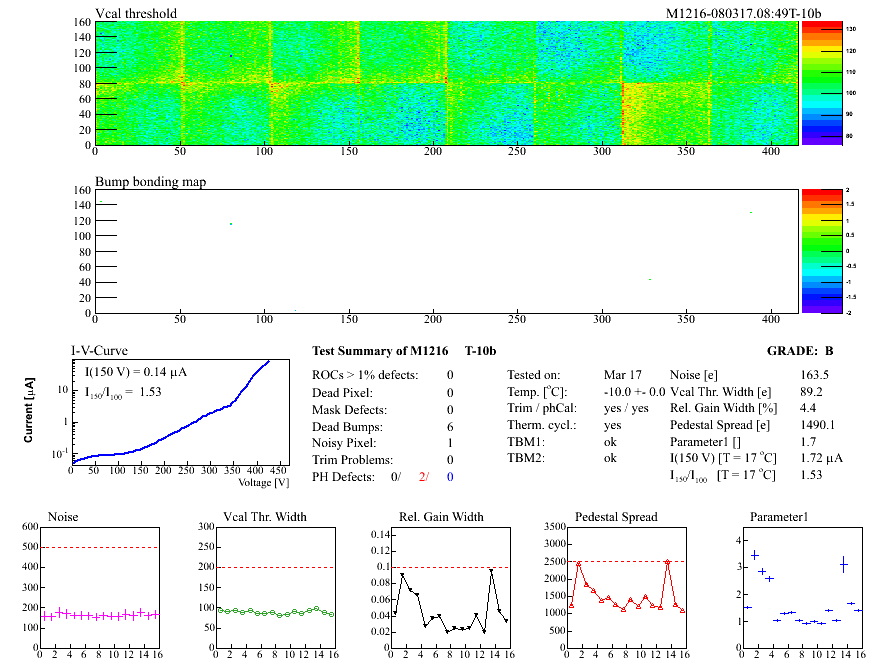
\includegraphics[width=160mm]{Content/Graphics/4_5_ModuleOverview.png}
						\caption{BPIX Module Testing Module Test Overview}
						\label{fig:AnalysisOfExistingApplicationBPIXModuleTestingModuleOverview}
					\end{figure}
					\begin{figure}[h!]
						\centering
						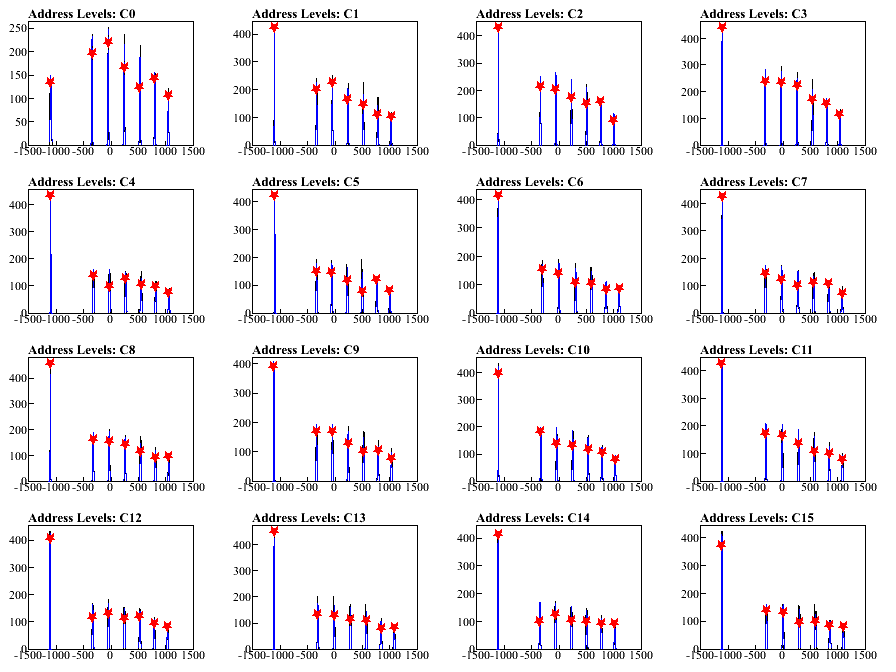
\includegraphics[width=160mm]{Content/Graphics/4_3_AddressLevels.png}
						\caption{BPIX Module Testing Module Address Levels}
						\label{fig:AnalysisOfExistingApplicationBPIXModuleTestingAddressLevels}
					\end{figure}
					\begin{figure}[h!]
						\centering
						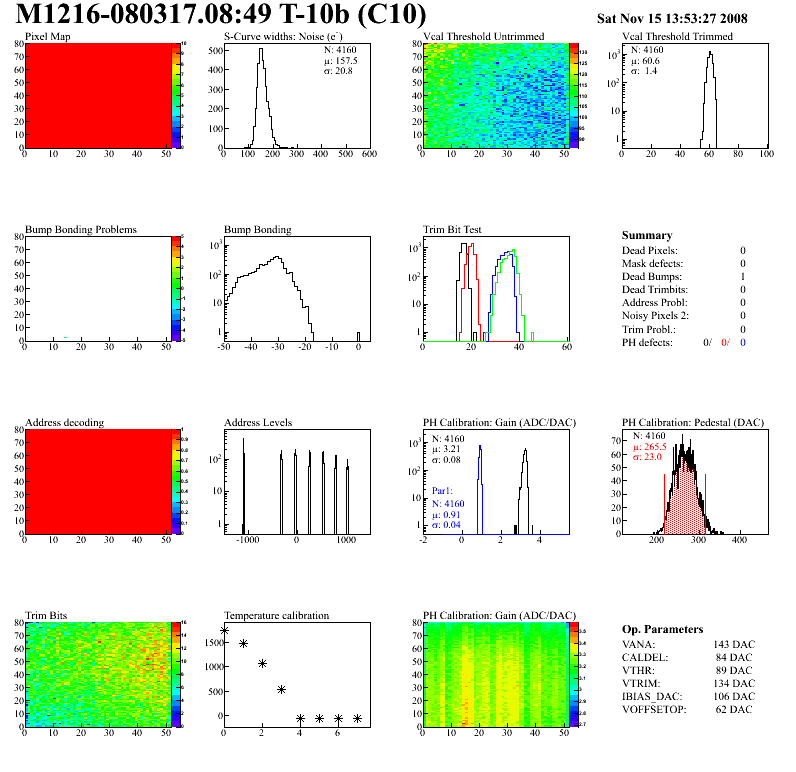
\includegraphics[width=160mm]{Content/Graphics/4_4_ROCTest.png}
						\caption{BPIX Module Testing ROC Test}
						\label{fig:AnalysisOfExistingApplicationBPIXModuleTestingROCTest}
					\end{figure}
					
				\paragraph{Source}
					The script located at \myPath{moduleTests/moduleDB/prodTable.php} generates the overview table seen in figure \ref{fig:AnalysisOfExistingApplicationBPIXModuleTestingModuleOverview}.
					It basically scans the \myPath{moduleTests/moduleDB/} and compares parts of the file or folder names to some parameters (e.g. series or search string). It parses the \myPath{summaryTest.txt} file of a module test and retrieves information such as test date, module number, grading, etc. from it.
			\subsubsection{Analysis Scripts}
			The analysis scripts that process the testing data an generate graphs etc. are located in \myPath{/home/peller/sdvlp/elcommandante/trunk/fitting} on the lion.ethz.ch server.
				\paragraph{Module Summary Page}
					The module summary page in figure \ref{fig:AnalysisOfExistingApplicationBPIXModuleTestingModuleOverview} is generated by the script \myPath{moduleSummaryPage.C}
					Some important functions are listed below:
					\begin{itemize}
						\item \function{moduleSummary} \\
							Generates an image file for the module summary page. 
							Generates the subplots using other functions in the file. Reads the data from ROOT-files. Saves the module summary as a .ps and .png file. Also generates the address level fits as .ps and .png files.
						\item \function{addVcalThreshold} \\
							Adds a Vcal Threshold diagram for a single chip to the Vcal Threshold overview.
						\item \function{makePlot} \\
							Draws the subplots ``Noise",``Vcal Thr. Width",``Rel. Gain Width",``Pedestal Spread",``Parameter1".(See fitNames, nfit variables in moduleSummary())
						\item \function{grading} \\
							Calculates grading for a module.
						\item \function{qualification} \\
							Calculates the number of dead pixels, etc. needed for grading.
						\item \function{fitPeaks} \\
							Finds peaks for chips in subplots and calculates some statistical values.	
					\end{itemize}
					The code is difficult to understand, since its structure is not obvious and it lacks documentation and comments.
				\paragraph{Chip Summary Page}
					The chip summary page in figure \ref{fig:AnalysisOfExistingApplicationBPIXModuleTestingROCTest} is generated by the script \myPath{chipSummaryPage.C}
					Some important functions are listed below:
					\begin{itemize}
						\item \function{chipSummary} \\
							Generates an image file for the chip summary page. 
							Generates the subplots using other functions in the file. Reads the data from ROOT-files. Saves the module summary as a .ps and .png file. 
						\item \function{analyse} \\
							Generates plots like ``ADC Measurement for ROC'', ``ADC Calibration for ROC'', etc.
						\item \function{readCriteria} \\
							Reads data like ``NOISE B'',``TRIMMING B'', etc. from a file.
					\end{itemize}
					The code is difficult to understand, since its structure is not obvious and it lacks documentation and comments.
		\subsection{Requirements}
			\subsection{General}
				 In general, MoRe-Web should be an easy-to-use interface for accessing information. It should be accessible by any client device and therefore be built on open web technologies. Furthermore, it should be optimized for display on mobile devices such as smart phones or table computers. All data should be stored in such a way that it can easily be accessed and processed by other software. 
				 It also is important that the code is easy to understand and maintain.
				 Furthermore, the software should be extensible and flexible, in order to meet requirements that might come up in the future.
			\subsection{Overview}
				The MoRe-Web should provide an overview list of all tested modules. There might be several tests per module. This should include a sortable and searchable list with additional information available by clicking or hovering an entry, as well as filtering options.
				By clicking a module, the module overview together with a list of the ROCs should be displayed, similar to the existing application (see figure \ref{fig:AnalysisOfExistingApplicationBPIXModuleTestingROCOverview}).
			\subsection{Module Test Overview}
				The overview page should offer information similar to figure \ref{fig:AnalysisOfExistingApplicationBPIXModuleTestingModuleOverview}
			\subsection{Module Test Details}
				In general, the test details should be available separately and offline, that is even without connection to MoRe-Web.
				The test detail page displays several plots for the test, which should be zoomable. The information available should be similar to the one in figure \ref{fig:AnalysisOfExistingApplicationBPIXModuleTestingROCTest}.
				It should also be possible to compare several tests of the same module.
		\subsection{Concept}
			The project is divided into two parts. First, the analysis scripts which are the connection point between the raw testing data and further processing. And second the web interface MoRe-Web.
			\subsubsection{Analysis Scripts}
				The analysis scripts should take data from ROOT-files and generate the following objects for both the module summary and the chip summary in the given directory structure:
				\begin{itemize}
					\item plots of test results
					\item HTML-file for summary pages which includes all plots and information and is accessible offline, that is it should be viewable directly from the file structure
				\end{itemize}
				Furthermore, the analysis scripts should insert the parsed data to a database system. For this particular case the use of sqlite is recommended, since no database server is needed and the database is directly stored in a file. Already existing entries will be replaced if the module number and the test date match.
				Since this database file is also available offline, it is used to generated an offline overview page.
			\subsubsection{MoRe-Web}
				The web interface is basically just a dynamic output of the overview page generated by the analysis scripts. The individual module tests consist of the offline HTML-files generated by the analysis scripts.
		\subsection{Implementation}
			\subsubsection{Analysis Scripts}
				The analysis scripts themselves are based on the following two abstract python classes, located in \myPath{AbstractClasses/}:
				\begin{itemize}
					\item \myPath{GeneralTestResult}
						This class is the base for the abstracted test classes for the module summary page, the chip summary page and the address levels. \\ 
						It provides functions for populating the data from raw result files, etc.
						For analysing a single module, a test result object is created out of the GeneralTestResult class, which in turn contains sub test result objects that again may store sub test result objects and so on. The hierarchy is shown in figure \ref{fig:ClassHierarchy}.
						\begin{figure}[h!]
							\centering
							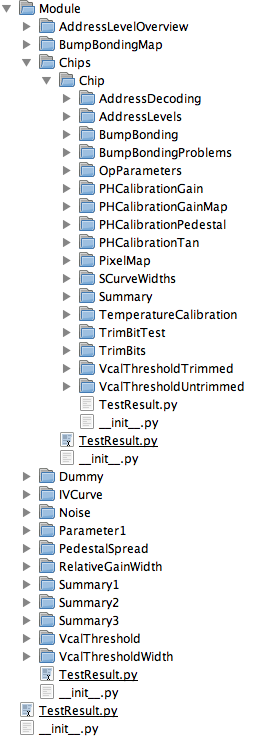
\includegraphics[width=60mm]{Content/Graphics/4_6_ClassHierarchy.png}
							\caption{Class Hierarchy for the inherited GeneralTestResult classes}
							\label{fig:ClassHierarchy}
						\end{figure}
						
						The actual test result data is structured in the following way:
						\begin{itemize}
							\item \function{Attributes} \\
								Hash table with attributes for the test, e.g. test date, tested object ID, module version, etc.
								
							\item \function{ResultData} \\
								\begin{itemize}
									\item \function{KeyValueDictPairs} \\
										Hash table that stores hash tables for unique keys containing a value, a unit and a label.
										For example a key can be ``TestTemperature'', and the correspoding hash table stores $-10$ as the value, \unit{\circ C} as the unit and ``Test Temperature'' as the label.
									\item \function{Plot} \\
										Hash table that stores a ROOT-Object used for the plot, a caption, a path to the generated image file and a file format.
									\item \function{SubTestResults} \\
										Hash table that stores sub test results, indexed by keys. For example, the module test result contains the IV-Curve as a sub test result.
									\item \function{Table} \\
										Hash table with three lists for header, body and footer data in a table.
								\end{itemize}
						\end{itemize}
						All the above data can be accessed by any test result object (therefore also by sub test results) since each test result object contains a reference to its parent test result object and the sub test results are indexed by a unique key. \\
						Some important functions implemented in the class are listed below:
						\begin{itemize}
							\item \function{PopulateAllData} \\
								This function invokes the data population for the rest results and all sub test results. It needs to be called for the topmost test result instance only.
							\item \function{CustomInit} \\
								Can be implemented for each test result class individually to set the name, some attributes and other variables before populating data.	
							\item \function{GetUniqueID} \\
								Returns a unique id for a ROOT-object in order to prevent memory problems.
							\item \function{GetPlotFileName} \\
								Returns the full path to the corresponding plot file for the current test result.
							\item \function{PopulateResultData} \\
								Implements how the data is populated for the current test result. That is, it can populate attributes, generate a plot file, store key value pairs and a data table. 
							\item \function{WriteToDatabase} \\
								This function invokes the data upload to the database for the rest results and all sub test results. It needs to be called for the topmost test result instance only. Could be extended for storing all sub test results including all attributes, plots, key value pairs etc. (currently not needed, only module test result are written to database as a single row entry)
							\item \function{CustomWriteToDatabase} \\
								Implements how the data is uploaded to the database for each test result.
						\end{itemize}
						Moreover, it implements several functions for generating the HTML-output, explained in detail in section \ref{sec:HTML-Output}
						For most test result classes, it is sufficient to implement the functions \function{CustomInit}  and \function{PopulateResultData}.
					\item \myPath{TestResultEnvironment}
						This class provides general functions and variables that are needed by all test results, such as database connectivity and general parameters. 
						The actual test result data is structured in the following way:
						\begin{itemize}
							\item \function{GradingParameters} \\
								Hash table with grading parameters used to calculate the final grade of a module.
								The grading parameters are read form a configuration file.
							\item \function{Configuration} \\
								Hash table containing several configuration parameters.
						\end{itemize}
				\end{itemize}
			\subsubsection{HTML-Output}
				\label{sec:HTML-Output}
				\paragraph{Test Result HTML File}
					As mentioned before, every test result object based on the class \function{GeneralTestResult} creates an output HTML-file for directly opening the test result data, such as plots, values, etc. 
					It contains a function called \function{GenerateDataFileHTML} which generates the output HTML file with the result data HTML obtained by calling \function{GenerateResultDataHTML} for the test result data and the sub test results. The functionality in \function{GenerateResultDataHTML} could also be directly implemented in \function{GenerateDataFileHTML}, but then it would not be possible to reuse it for sub test results that are displayed on the same page. For example, the module overview page contains a data table with all ROCs, but also several subtests, which are displayed on the same page. 
					As of functionality, there are some key features worth mentioning:
					\begin{itemize}
						\item \textbf{Navigation} Since there are references to parent and sub test results in each test result instance, a relative navigation between the test results can be implemented without connection to a database at runtime. 
						\item \textbf{Style} The styling of the HTML document is done using CSS. The layout adapts to different display sizes by dynamically adapting the number of columns shown to the screen width. Therefore it is also possible to browse the files on a mobile device.
						\item \textbf{Template} The HTML-files are generated using template files by replacing markers with actual content. Hence the layout can be changed without changing the code. For this, the templating class of the TYPO3-Project (\url{www.typo3.org}) was ported to python and can be found at \myPath{AbstractClasses/Helper/HTMLParser.py}
					\end{itemize}
				\paragraph{Overview HTML File}
					Using the same styling, layout and templating as in the test result HTML-files, an overview page is generated using the class \function{ModuleResultOverview}, which reads the data from either the local database or the global database.
		\subsection{Controller}
			A module qualification session is instantiated using the \myPath{Controller.py} program.
			It will instantiate the module test result object for all folders found in the \function{TestResultDirectory} variable defined in the configuration and all necessary sub test result objects from the classes found in \myPath{TestResultClasses/CMSPixel/ModuleTestGroup/}, provide it with a test result environment object containing data relevant for the qualification session. It also reads the configuration and sets all relevant paths.
			\subsubsection{System Requirements}
				The following requirements have to be met in order for the Controller.py to run correctly:
				\begin{enumerate}
					\item Python installed, minimum version: $2.7$
					\item Python packages:
						\begin{enumerate}
							\item ROOT (\url{http://root.cern.ch/drupal/content/pyroot})
							\item Python packages:
								
						\end{enumerate}
				\end{enumerate}
			
			\subsubsection{Step-By-Step Guide}
				Follow this step-by-step guide in order to perform module qualifications and generate the result output.
				\begin{enumerate}
					\item Check the minimum requirements as described in section \ref{sec:ControllerMinimumRequirements}
					\item Open the command line on your UNIX system(Mac, Linux, etc.)
					\item Change to the directory where the analysis scripts are located by typing \commandline{cd PathToAnalysisScripts}, where you replace \commandline{PathToAnalysisScripts} by the actual path to the analysis scripts.
					\item Adjust the configuration to your current qualification session by editing the configuration files found in the \myPath{Configuration/} subfolder. The following lists describes the content of each configuration file:
						\begin{itemize}
							\item \textbf{GradingParameters.cfg} Contains all the grading parameters. Usually needs no changes.
							\item \textbf{ModuleInformation.cfg} Contains module information such as the module version, etc. for the type of modules analysed in the current qualification session.
							\item \textbf{Paths.cfg} Stores the paths to the test result directory where all test results you want to qualify in this session are stored. Moreover, the path to the overview page is stored. This directory also contains the local \myPath{Overview.sqlite} sqlite database that stores all qualification results. The same database can be used for any number of qualification sessions, even when the test results in each session are stored in different folders, and therefore the resulting overview page contains all module qualification results. 
							\item \textbf{SystemConfiguration.cfg} Several system parameters such as the default image format, database connection parameters, etc. can be changed in this file.
						\end{itemize}
					\item Type the command \commandline{python Controller.py} to run the qualification session. For each module, it should display \\
					``Working on:  {'TestDate': '1363355666', 'TestType': 'FullQualification', 'ModuleID': 'M1193'} --''. The current step is shown as either ``Populating Data'' or ``Generating Final Output''. If other messages occur, it is recommended to analyse their meaning, as they are most probably indicating some problems that might have occured during the qualification process.
 					\item If no error messages appeared, all files should have been generated and the overview page can be found in the folder specified in the configuration. Each module test result folder now contains a folder called \myPath{FinalResults}, which you can browse to access the test result files of any sub test. \textbf{Important Notice:} The HTML-files can be opened with any web browser, but for best results, make sure you use an up-to-date version of one of the applications recommended in table \ref{tab:BrowserRecommendations}. Please note that Internet Explorer lower than version $10$ is unable to display SVG-graphics. If needed, the output file format can be changed to ``png'', with the drawback of using the scalability of vector graphics.
 					\begin{table}[h]
						\centering
						\begin{tabular}[c]{l|r}
							Application	& Minimum Version\\
							\hline
							Mozilla Firefox 	& $4$ \\
							Google Chrome 	&  $18$ \\
							Safari 		& $3$ \\
							Opera 		&  $9$ \\
							Internet Explorer 	&  $10$ \\
						\end{tabular}
						\label{tab:BrowserRecommendations}
						\caption{Browser recommendations for opening the HTML-files}
					\end{table}
				\end{enumerate}
				
				
				python minimum requirement: 2.7
				
				
\end{document}
